\documentclass[twocolumn]{revtex4-2}
\usepackage{amssymb, amsfonts, physics, bm, graphicx, tikz}
\renewcommand{\arraystretch}{1.5}

\begin{document}

\title{M-Sequences from Galois Fields}
\thanks{Matthew Rowe (\today)}

\begin{abstract}
Just enough finite field theory to understand some properties of maximum length sequences (hereafter called M-sequences). 
This document is not concerned with proofs or rigour; it is very much a `roughly speaking' take on the subject.
Knowledge of basic finite group theory is assumed and the presentation leans heavily on David Forney's MIT course \emph{Principles of Digital Communication II}.
\end{abstract}

\maketitle

\section{Finite Field Theory}
A \emph{field} $\mathbb{F}$ is set $S$ endowed with operations $+$ and $\cdot$ such that $\{S, + \}$ and $\{S \backslash \{0\}, \cdot \}$  are abelian groups with identity elements $0$ and $1$ respectively.
There is also the constraint that the operations mesh nicely with each other $a \cdot (b + c) = a \cdot b + a \cdot c$. Examples of infinite fields are $\mathbb{R}, \mathbb{C}$ and $\mathbb{Q}$.
We shall be concerned with finite fields, the simplest of which are the numbers mod-$p$ for $p$ prime. That is $\{0,1,\ldots,p-1\}$ under normal addition and multiplication modulo $p$.
We denote this $\mathbb{F}_p$. In fact, as we shall discuss later, all finite fields must be of the form $\mathbb{F}_{p^n}$ for some $n$, and these have $\mathbb{F}_p$ as a subfield.
All fields of a given size are isomorphic. It is also convenient to define the \emph{characteristic} of a field as the smallest number $k$ for which $1+1+\cdots+1$ ($k$ times) equals $0$. 
This never happens for infinite fields and they are said to have characteristic $0$. Finite fields have characteristic $p$.

\subsection{Polynomials over $\mathbb{F}$}
Define $\mathbb{F}[X]$ as the set of all polynomials of the form
\begin{equation}
    f(X) = f_0 + f_1 X + \ldots + f_m x^m
\end{equation}
where $f_i \in \mathbb{F}$ and $X$ is formally just a symbol. Here $m$ is the degree of the polynomial and addition and multiplication of polynomials is `as usual' with modular arithmetic for the coefficients.
As multiplication tends to increase the degree of polynomials, all non-zero degree polynomials have no multiplicative inverse. 
Division is thus tricky and for this reason $\mathbb{F}[X]$ is an algebraic structure called a \emph{ring} rather than a field. A polynomial is called \emph{monic} if its highest coefficient $f_m = 1$.

A polynomial $g(X)$ is called a \emph{divisor} of $f(X)$ if $f(X) = q(X) g(X)$ for some quotient $q(X)$. Trivial divisors are $1$ and $f$ itself. 
Slightly more specifically a divisor is a \emph{factor} if it is monic and non-trivial. A $m>0$ degree polynomial that has no factors is called \emph{irreducible}. 
Remember the coefficients of the factors must be in $\mathbb{F}$, for finite fields no nasty square roots are allowed!
There is a \emph{unique factorisation} theorem that we shall not prove: every polynomial in $\mathbb{F}[X]$ may be written as a unique product of monic irreducible polynomials (times a constant).
These monic irreducible polynomials, sometimes called prime polynomials, are analogous to the primes in $\mathbb{Z}$.

Consider a monic $g(X)$ of degree $m$. Any $f(X)$ can be decomposed as
\begin{equation}
f(X) = q(X) g(X) + r(X)
\end{equation}
for unique $q$ and remainder $r$, with $\text{deg}(r) < m$. With this we can define mod-$g(X)$ addition and multiplication of polynomials.
That is, the result of operations modulo $g(X)$ are in terms of the remainders. 
Note that for coefficients in $\mathbb{F}_p$ the size of the remainder set generated by mod-$g(X)$ operations is $|\mathbb{F}_p|^m$.

\subsection{Fields $\mathbb{F}_{g(X)}$}
With modulo $g(X)$ operations we can construct a field out of the set of remainder polynomials. Let $\mathbb{F} = \mathbb{F}_p$ and $g(X) \in \mathbb{F}_p[X]$ be a degree $m$ irreducible, monic polynomial.
The set of remainder polynomials under mod-$g(X)$ addition and multiplication has $p^m$ elements of the form
\begin{equation}
    r_0 + r_1 X + \ldots + r_{m-1} X^{m-1} \, , \qquad r_j \in \mathbb{F}_p
\end{equation}
which (one can prove) forms a field. As all finite fields are isomorphic this is \emph{the} finite field $\mathbb{F}_{p^m}$.

For example, consider $m=2$ polynomials over $\mathbb{F}_2$. The polynomial $g(X) = X^2 + X + 1 \in \mathbb{F}_2[X]$ is irreducible and monic and so we can form the remainder set.
These are degree $0$ and $1$ polynomials, i.e. $\{0,1,X, X+1\}$ which form $\mathbb{F}_{2^2}$. This is closed as for example $X \cdot X$ modulo $(X^2 + X + 1)$ is $X + 1$.

\subsection{Roots and Cyclicity of $\mathbb{F}^*_q$}
If $f(x) \in \mathbb{F}[X]$ has a factor $X - a$ then $a$ is a \emph{root} of $f(X)$, i.e. $f(a) = 0$. 
The fundamental theorem of algebra states that a monic polynomial of degree $k$ can have at most $k$ roots in $\mathbb{F}$. If $\mathbb{F} = \mathbb{C}$ then it has exactly $k$ roots.

We now take another view on the field $\mathbb{F}_q$, for some finite $q$. We cast aside our knowledge that $q= p^n$ and ignore polynomials for now. 
Define $\mathbb{F}^*_q = \mathbb{F}_q \backslash \{0\}$ and consider any element $\beta \in \mathbb{F}_q^*$. Keep multiplying it by itself $\beta, \beta^2, \ldots$, eventually we must return to $1$ (as this is a finite field).
This thus generates a cyclic group $\{1, \beta, \beta^2, \ldots , \beta^{l-1}\}$ whose size $l$ must divide the abelian group $(\mathbb{F}_q^*, \cdot)$ by Lagrange's theorem. Thus $\beta^l = 1$ and by extension
\begin{equation}
    \beta^{q-1} = 1 \text{ for all } \beta \in \mathbb{F}_q^* \, .
\end{equation}
Thus all of the $\beta \in \mathbb{F}_q^*$ are distinct roots of the polynomial $X^{q-1}-1 \in \mathbb{F}_q[X]$.
Equivalently, including $0$, all $\beta \in \mathbb{F}_q$ are roots of $X^q - X$ which can therefore be factored as
\begin{equation}
    X^q - X = \prod_{\beta \in \mathbb{F}_q} (X - \beta) \, .
\end{equation}
Some $\beta$ are special in that they generate the whole group (i.e. $l=q-1$). These are called primitive elements which we conventionally denote $\alpha$. At least one always exists.
Consequently a finite field can be written
\begin{equation}
    \mathbb{F}_q = \{0,1,\alpha, \alpha^2, \ldots , \alpha^{q-2}\}
\end{equation}
where $\alpha$ is primitive. $\mathbb{F}_q^*$ is a cyclic group of order $q-1$ generated by $\alpha$. For example $\mathbb{F}_{2^4} = \{0, 1, \ldots , \alpha^{14} \}$ with elements $\{\alpha^5, \alpha^{10}\}$ of order $3$,
$\{ \alpha^3, \alpha^6, \alpha^9, \alpha^{12} \}$ of order $5$. The remaining $8$ elements are primitive (order $15$).

\subsection{$\mathbb{F}_q^*$ as Polynomials}
We previously had the remainder field $\mathbb{F}_{g(X)}$ of polynomials with coefficients in $\mathbb{F}_p$. We have just constructed a general field $\mathbb{F}_q$ in terms of primitive elements.
The link between the two viewpoints is the following theorem, stated without proof:
\begin{quote}
Every finite field $\mathbb{F}_q$ of characteristic $p$ is isomorphic to the polynomial remainder field $\mathbb{F}_{g(X)}$ derived from an $m^{\text{th}}$ degree monic irreducible polynomial $g(X) \in \mathbb{F}_p[X]$.
By size, therefore, $q = p^m$ for some $m$.
\end{quote}
As before the polynomial $X^{p^m} - X$ may be factorised into its roots $x-\beta$ for every $\beta \in \mathbb{F}_{p^m}$. 
Further however we can prove that every $m^{\text{th}}$ degree (monic) irreducible polynomial in $\mathbb{F}_p[X]$ divides this polynomial. Thus we also a guaranteed another factorisation of $X^{p^m}-X$.
\begin{quote}
The polynomial $X^{p^m}-X \in \mathbb{F}_{p^m}[X]$ can be written as a product of all monic irreducible polynomials in $\mathbb{F}_p[X]$ of degree $m$ or a number that divides $m$, without repetition.
\end{quote}
Irreducible polynomials are all very good, but can we do better? An irreducible polynomial $g(X) \in \mathbb{F}_p[X]$ of degree $m$ that has a primitive element, $\alpha \in \mathbb{F}_{p^m}$, as a root is known a \emph{primitive polynomial}.
More formally primitive polynomials are minimal polynomials of primitive elements. Given a primitive $\alpha$, its \emph{minimal} polynomial is the lowest degree monic polynomial (in $\mathbb{F}_p[X]$) that has $\alpha$ (in $\mathbb{F}_{p^m}$) as a root.
It is important to stress that primitive $g(X)$ is not a field element; it generates the remainder field $\mathbb{F}_{g(X)}$ of degree $m-1$ polynomials. Under the isomorphism $\mathbb{F}_{p^m} \cong \mathbb{F}_{g(X)}$ the primitive element $\alpha \longleftrightarrow X \text{ modulo }g(X)$.
We care a lot about primitive polynomials as all of their roots are primitive elements and thus generate the group: indeed (unproven) if the original $\alpha$ is a root, so is $\alpha^p, \alpha^{p^2}, \ldots , \alpha^{p^{m-1}}$ also all primitive.
For a given $m$ there are $\varphi(p^m - 1)/m$ different primitive polynomials to choose from, where $\varphi(n)$ is Euler's totient function (the number of integers coprime to $n$).
That is, there are $\varphi(p^m - 1)$ primitive elements, and each primitive polynomial corresponds to $m$ of these ($m$ roots). Examples of binary primitive polynomials are given in Table \ref{tab:primitivepoly} below.
\begin{table}[ht] 
\centering 
\begin{tabular}{c c} 
\hline
Degree $(n)$ & $g(x)$ \\ 
\hline
1 & $x + 1$ \\ 
2 & $x^2 + x + 1$ \\ 
3 & $x^3 + x + 1$ \\ 
4 & $x^4 + x + 1$ \\ 
5 & $x^5 + x^2 + 1$ \\ 
6 & $x^6 + x + 1$ \\ 
7 & $x^7 + x + 1$ \\ 
8 & $x^8 + x^6 + x^5 + x + 1$ \\
\hline 
\end{tabular} 
\caption{Primitive polynomials over $\mathbb{F}_2$ of degree $n$ (non-exhaustive)} 
\label{tab:primitivepoly} 
\end{table}

\subsection{Addition of Field Elements}
\label{sec:logarithms}
So far we have talked a lot about multiplication. This is easy in terms of primitive elements, $\alpha^i \cdot \alpha^j = \alpha^{i+j}$, but what about addition $\alpha^i + \alpha^j$?
This is $\alpha^k$ for some $k$, but what $k$? To save laborious computations one usually looks up the result in a `logarithm' table.
For a primitive element $\alpha$, define the \emph{Zech logarithm} as
\begin{equation}
    Z_\alpha(n) = \log_{\alpha}(1+\alpha^n)
\end{equation}
or more properly the solution to $\alpha^{Z_\alpha(n)} = 1 + \alpha^n$. This enables addition to be done quickly
\begin{equation}
    \alpha^i + \alpha^j = \alpha^i ( 1 + \alpha^{j-i}) = \alpha^{i + Z_{\alpha}(j-i)} \, .
\end{equation}
For characteristic $p=2$ (binary) fields this has an `involution' type property
\begin{equation}
    Z_\alpha(n) = m \quad \Longleftrightarrow \quad Z_\alpha(m) = n
\end{equation}
which is easily proved by noting 
\begin{equation}
\alpha^{Z(Z(n))} = 1 + \alpha^{Z(n)} = 1 + 1 + \alpha^n = \alpha^n \quad \text{mod-}2.
\end{equation}

\subsection{Vector Spaces and Traces}
The final element we must cover before turning to M-sequences is the concept of finite field traces. In linear algebra the trace is the (basis independent) sum of a matrix's diagonal elements, but how do we get to there from finite fields?
The answer really has been staring us in the face all along: $\mathbb{F}_{p^m}$ naturally forms a vector space with coefficients in the subfield $\mathbb{F}_p$.
This is most easily seen from the polynomial remainder field interpretation, $\mathbb{F}_{g(X)} \cong \mathbb{F}_{p^m}$. The `vectors' are the polynomials with normal polynomial addition and scalar multiplication (mod-$p$).
Note that while $\mathbb{F}_{p^m}$ \emph{can} be viewed as a vector space its structure is richer, being a field, due to the ability to multiply the `vectors'.

The set $\{1, X, X^2, \ldots , X^{m-1}\}$ forms a basis for this space with specific elements represented as tuples / coordinates $(a_0, a_1, \ldots, a_{n-1})$ with $a_i \in \mathbb{F}_p$.
We can then define linear maps on this space, represented by matrices. Consider the map which is a simple multiplication by some element $\beta \in \mathbb{F}_{p^m}$, i.e. $x \to \beta x$. Denote this as $m_\beta : \mathbb{F}_{p^m} \to \mathbb{F}_{p^m}$. 
This takes an input tuple and maps it to another tuple and thus has a corresponding matrix $M_\beta$.
For example consider $\mathbb{F}_{2^3}$ with $g(X) = X^3 + X + 1$ and multiplication by $\beta = 1 + X$. This maps the basis
\begin{alignat}{2}
    1 &\longrightarrow 1+X \nonumber \\[0.1cm]
    X &\longrightarrow X + X^2 \\[0.1cm] 
    X^2 &\longrightarrow X^2 + X^3 = X^2 + X + 1, \nonumber
\end{alignat}
which has matrix representation
\begin{eqnarray}
    M_\beta = \mqty(1 & 0 & 1 \\ 1 & 1 & 1 \\ 0 & 1 & 1) \, .
\end{eqnarray}
Note that in this case $g(X)$ was primitive but only irreducibility is required here. With this all in mind we can define the \emph{trace of a finite field element} $\beta \in \mathbb{F}_{p^m}$ as
\begin{equation}
\label{eq:tracedef}
    \Tr_{\, \mathbb{F}_{p^m}/\mathbb{F}_p}(\beta) \equiv \text{trace}(M_\beta)
\end{equation}
that is the trace of the linear map $x \to \beta x$ in the normal linear algebra sense. Correspondingly this is a linear operation. For the above example the trace is $3 = 1$ (mod-$2$).
The subscript $\mathbb{F}_{p^m}/\mathbb{F}_p$ is there to remind us that the trace is a map from the full $\mathbb{F}_{p^m}$ down to the prime subfield $\mathbb{F}_p$. We shall omit this henceforth.
While we shall not prove it one can show that \eqref{eq:tracedef} can alternatively be written as a sum of `conjugates' $\sum_{i=0}^{m-1} \beta^{p^i}$.


\section{M-Sequences}
We now know enough to properly define M-sequences. In the communications literature finite fields are usually referred to as \emph{Galois} Fields and denoted $\text{GF}(p^n)$ rather than $\mathbb{F}_{p^n}$.
The field $\text{GF}(p^n)$ is also often referred to as the \emph{extension} of the base field $\text{GF}(p)$.

\subsection{From Galois Fields}
Take the binary field $\text{GF}(2^n)$ parameterised in terms of some primitive element $\alpha$ and its corresponding minimal (primitive) polynomial $g(X)$.
M-sequences are constructed in terms of the trace of the extension field back into $\text{GF}(2) = \{0,1\}$. An M-sequence $s[i]$ is defined as
\begin{equation}
    s[i] \equiv \Tr(\alpha^i) \in \{0,1\} \, , \qquad i = 0, 1, \ldots
\end{equation}
which, as $\alpha$ is primitive, generates the entire field apart from the zero element. Thus M-sequences are of length $L=2^n-1$, periodically repeating after this as $\alpha^{2^n - 1} = 1$.
It is important that $\alpha$ is primitive, other elements would generate a sequence but it would not be of maximum length!

In digital applications M-sequences are typically defined as either 
\begin{equation}
m[i] \equiv (-1)^{s[i]} \qquad \text{or} \qquad m[i] \equiv 2s[i]-1 \, ,
\end{equation}
mapping to $\pm 1$ rather than $\{0,1\}$. The two definitions differ by a global minus sign.
Cyclic shifts of M-sequences just correspond to multiplication by some field element $\beta = \alpha^\tau$, that is $s[i+\tau] = \Tr(\beta \alpha^i)$. 
This gives the curious property that the product of an M-sequence with a shifted version of itself is \emph{also} an M-sequence at a \emph{different} offset. Using the first definition and the linearity of the trace
\begin{alignat}{2}
    m[i] \, m[i+\tau] &= (-1)^{s[i]+s[i+\tau]} \\[0.1cm]
    &= (-1)^{\Tr(\alpha^i) + \Tr(\alpha^{i+\tau})} \nonumber \\[0.1cm]
    & = (-1)^{\Tr(\alpha^i (1+ \alpha^\tau))} \nonumber \\[0.1cm]
    &= (-1)^{\Tr( \alpha^{i+Z_\alpha(\tau)})} \nonumber \\[0.1cm]
    & = m[i+ Z_\alpha(\tau)] \, , \nonumber 
\end{alignat}
the offset is in terms of the Zech logarithms defined in Section \ref{sec:logarithms}.

\subsection{As Recurrence Relations}
Consider the $n^{\text{th}}$ order primitive polynomial
\begin{equation}
    g(X) = g_0 + g_1 X + \cdots + g_{n-1} X^{n-1} + X^n \, ,
\end{equation}
arising from the primitive element $\alpha$. We have that $g(\alpha) = 0$ and thus $0 = \sum_i g_i \alpha^i$. Premultiplying by some offset $\alpha^\tau$ and taking the trace we get 
\begin{equation}
    0 = \sum_{i=0}^n g_i \, s[i+\tau] \qquad (\text{mod-}2)
\end{equation}
or rearranged, $s[n+\tau] = - \sum_{i=0}^{n-1} g_i s[i+\tau]$ for any $\tau$. 
We see that $s[n]$ is determined entirely by the $n$ previous values $s[0], \ldots, s[n-1]$ and by extension
\begin{equation}
\label{eq:mseqrecursion}
    s_i = -  \big( g_{n-1} s_{i-1} + g_{n-2} s_{i-2}
    + \cdots + g_0 s_{i-n} \big) |_{(\text{mod-}2)}
\end{equation}
changing notation for brevity. M-sequences can therefore equivalently be defined as an order $n$ \emph{recurrence relation} in terms of the primitive polynomial coefficients.
Initialising with $n$ binary values specifies the whole sequence. Barring $(0,\ldots,0)$ which will remain at $0$ there are $2^n-1$ possible initial conditions which generate cyclic shifts of the same M-sequence. 
Different M-sequences arise from different primitive polynomials, at order $n$ there are $\varphi(2^n-1)/n$ of these. Explicitly for $n=2,3, \ldots$ there are $1,2,2,6,6,18,16, \ldots$ unique sequences.
Note that the initial condition is often quoted as an integer seed arising from interpreting $(s_{n-1}, \ldots, s_{0})$ as a binary number. The same trick can also be done with the polynomial coefficients.

\subsection{From Shift Registers}
At any point $i$ in the sequence we can define the current \emph{state} as $(s_{i}, s_{i-1}, \ldots, s_{i-n+1})$, i.e. all the values required to calculate $s_{i+1}$.
Each step \emph{shifts} the state right
\begin{equation}
    (s_{i}, s_{i-1}, \ldots, s_{i-n+1}) \longrightarrow (s_{i+1}, s_{i}, \ldots, s_{i-n+2})
\end{equation}
where the new value $s_{i+1}$ comes from `feedback' from the previous values in a linear manner \eqref{eq:mseqrecursion}. 
This defines an (additive) linear-feedback shift register (LFSR) of length $n$. Over the course of the sequence all possible states of the shift register will be realised.

A graphical representation of a specific order $4$ sequence with primitive polynomial $X^4+X+1$ is shown in Figure \ref{fig:shiftregister}. 
Let $\{a_3, a_2, a_1, a_0\}$ denote the register values, initialised at $\{1,1,1,1\}$. Now shift everything to the right, sending $a_0 = 1$ to the output on the right. 
This is the first term in our order $4$ M-sequence. As we successively shift right the first $4$ outputs are $1,1,1,1$, i.e. the initial state of the register. 
The register values therefore satisfy $s[i] = a_r[i-r]$. For this primitive polynomial only $g_0$ and $g_1$ are non-zero meaning $s_{i} = - s_{i-3} -  s_{i-4}$ or equivalently $s_{i+4} = s_{i+1} + s_{i}$ (mod-$2$). 
In terms of register values this becomes $a_3[i+1] = a_1[i] + a_0[i]$ (mod-$2$) meaning the vacant space on the left of the register is filled with the XOR (modulo $2$ addition) of what was previously in $a_1$ and $a_0$ as shown in the diagram.
The first fill is therefore $1 \oplus 1 = 0$ and the second state of the register is $\{0,1,1,1\}$. We then repeat the process, sending $1$ to the output and another $0$ to the far left. 
This gives the pattern
\begin{alignat*}{2}
    \{1,1,1,1\} &\qquad \text{OUT}: 1 \nonumber \\[0.1cm]
    \{0,1,1,1\} &\qquad \text{OUT}: 1 \nonumber \\[0.1cm]
    \{0,0,1,1\} &\qquad \text{OUT}: 1 \nonumber \\[0.1cm]
    \{0,0,0,1\} &\qquad \text{OUT}: 1 \nonumber \\[0.1cm]
    \{1,0,0,0\} &\qquad \text{OUT}: 0 \nonumber \\[0.1cm]
    \{0,1,0,0\} &\qquad \text{OUT}: 0 \nonumber \\[0.1cm]
    \vdots \qquad& \qquad \qquad \vdots \nonumber
\end{alignat*}
This continues on until all possible $2^4 - 1$ configurations of the register have been exhausted ($\{0,0,0,0\}$ cannot be reached). 
The $15$ output values form the order $4$ m-sequence: $1,1,1,1,0,0,0,1,0,0,1,1,0,1,0$.
More complicated primitive polynomials will have multiple feedback `taps' and the shift register set up is more involved.
\begin{figure}[t]
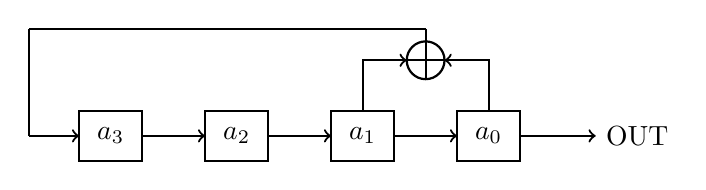
\begin{tikzpicture}[scale=0.8, thick]
\foreach \x/\lab in {0/a_3,2/a_2,4/a_1,6/a_0} { \draw (\x,-0.4) rectangle ++(1,0.8); 
\node at (\x+0.5,0) {$\lab$}; }
\draw[->] (-0.8,0) -- (0,0); 
\draw[->] (1,0) -- (2,0); 
\draw[->] (3,0) -- (4,0); 
\draw[->] (5,0) -- (6,0); 
\draw[->] (7,0) -- (8.2,0); 
\node[right] at (8.2,0) {OUT}; 
\draw (5.5,1.2) circle (0.3); 
\draw (5.2,1.2) -- (5.8,1.2); 
\draw (5.5,0.9) -- (5.5,1.5);
\draw[-] (-0.8,1.7) -- (-0.8,0); 
\draw (5.5,1.7) -- (-0.8,1.7); 
\draw (5.5, 1.2) -- (5.5, 1.7);
\draw[->] (4.5, 0.4) -- (4.5, 1.2) -- (5.2, 1.2);
\draw[->] (6.5, 0.4) -- (6.5, 1.2) -- (5.8, 1.2);
\end{tikzpicture}
\caption{An example linear feedback shift register of length $4$. The $\oplus$ represents addition modulo $2$.}
\label{fig:shiftregister}
\end{figure}

\subsection{Autocorrelation}
The most famous property of M-sequences is their impulsive circular autocorrelation and thus flat power spectrum (by the Wiener-Khinchin Theorem).
Consider again $\text{GF}(2^n)$ as a $n$-dimensional vector space over $\{0,1\}$ with the M-sequence defined as a linear map (specifically the trace) on this space. 
M-sequence values of $0$ therefore correspond to elements in the nullspace (kernel) of this map. 
The image of the map is $\{0,1\}$, which has dimension $1$ and so by the Rank-Nullity Theorem the kernel has dimension $n-1$.
Consequently a trace of $0$ appears $2^{n-1}$ times and thus a trace of $1$ also appears $2^n - 2^{n-1} = 2^{n-1}$ times: this is the \emph{balance} property.
However be careful to note that the field's $0$ element (the additive identity which has trace $0$) is excluded from the sequence so the M-sequence itself has one more $1$ than $0$.
Thus $\sum_{i=0}^{L-1} m[i] = -1$. This allows us to determine the autocorrelation of two length-$L$ M-sequences. For $i \neq0$
\begin{alignat}{2}
    (m \circledast m)[i] &= \sum_{k=0}^{L-1} m[k]^* m[(k+i)_{\text{mod-}L}] \\[0.1cm]
    &= \sum_{k=0}^{L-1} (-1)^{\Tr(\alpha^k)} \cdot (-1)^{\Tr(\alpha^{k+i})} \nonumber \\[0.1cm]
    &= \sum_{k=0}^{L-1} (-1)^{\Tr(\alpha^k \alpha^{Z_\alpha(i)})} \nonumber \\[0.1cm]
    &= \sum_{k=0}^{L-1} m[k + Z_\alpha(i)] = -1 \nonumber \, ,
\end{alignat}
as for any fixed $i$ the $Z_\alpha(i)$ is just a cyclic shift. At $i=0$ the sum reduces to $\sum_k m[k]^2 = \sum_{k} 1 = L$ and thus
\begin{equation}
    (m \circledast m)[i] = \Bigg\{
    \begin{array}{cc}
        L, & \qquad i=0, \\
        -1, & \qquad \text{otherwise}.
    \end{array}
\end{equation}
Impulsive autocorrelations are an important property of truly random sequences. 
Of course M-sequences are deterministic, but for this reason they are referred to as a type of pseudorandom binary sequence (PRBS).


\end{document}